\documentclass{beamer}
\usetheme{Madrid}

\usepackage{amsmath}
\usepackage{graphicx}
\usepackage{multicol}
\usepackage{multirow}
\usepackage{array}

\usepackage{tikz}
\usetikzlibrary{shapes.geometric, arrows}
\usetikzlibrary{calc}
\usetikzlibrary{matrix, positioning}

\tikzstyle{matrix of math nodes}=[
  matrix of nodes,
  % nodes in empty cells,
  column sep=-\pgflinewidth,
  row sep=-\pgflinewidth,
  nodes={draw,
    minimum size=2em,
    anchor=center,
    inner sep=0pt,
    execute at begin node=$,
    execute at end node=$
  }
]

\usepackage{pgfplots}
\pgfplotsset{compat=1.18}

\pgfplotsset{
    report_style/.style={
    legend style={draw=none, font=\small},
    legend cell align=left,
    legend pos=north east,
    ylabel style={align=center, font=\bfseries\boldmath},
    xlabel style={align=center, font=\bfseries\boldmath},
    x tick label style={font=\bfseries\boldmath},
    y tick label style={font=\bfseries\boldmath},
    scaled ticks=false,
    every axis plot/.append style={thick},
    },
}

\usepackage[justification=centering]{caption}
\usepackage{subcaption}

\usepackage{xurl}

% default path to images and other assets
\graphicspath{{../assets/}}

% disable wrapping
\tolerance=1
\emergencystretch=\maxdimen
\hyphenpenalty=10000
\hbadness=10000

% number figure caption
\setbeamertemplate{caption}[numbered]

% display bib label in references
\setbeamertemplate{bibliography item}{\insertbiblabel}
\setbeamertemplate{bibliography entry title}{}
\setbeamertemplate{bibliography entry location}{}
\setbeamertemplate{bibliography entry note}{}

\newcommand{\fall}[1]{\quad \textcolor{red}{#1}}

% Metadata
% ------------------------
\title[Connectomics segmentation]{Segmentation of 3D volume images for connectomics}
\subtitle{CMS Research project}

\author[Oleh Shkalikov]{Oleh Shkalikov\texorpdfstring{ (5102818)
\\[0.7em]{\small Supervisors: Jannik Irmai, David Stein}
\\{\small Chairholder: Prof. Dr. Bjoern Andres}}{}}

\institute[TU Dresden]{TU Dresden, MLCV chair}

\date{14 March, 2024}

\begin{document}

\frame{\titlepage}

% \begin{frame}
%     \frametitle{Agenda}
%     \tableofcontents
% \end{frame}

\section{Dataset description and analysis}
\begin{frame}
    \frametitle{The original dataset}
    \begin{minipage}{0.49\textwidth}
        The original image volumes are acquired by a focused ion beam scanning electron microscope (FIB-SEM)
        of the CA1 hippocampus region of the brain.
        The raw data has a shape \( 2048 \times 1536 \times 1065 \) and initially were used by
        \cite{lucchi2013learning,lucchi2011supervoxel} for mitochondria segmentation task.
    \end{minipage}
    \begin{minipage}{0.49\textwidth}
        \centering
        \begin{figure}
            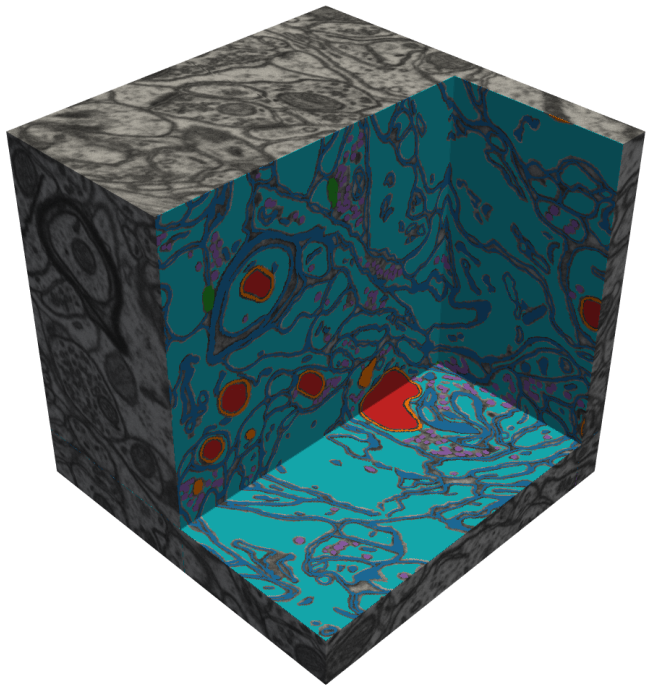
\includegraphics[width=0.8\textwidth]{cube_labeled.png}
            \caption{Connectomics volume image with provided labels\footnote{Credits to Jannik Irmai}}
        \end{figure}
    \end{minipage}
\end{frame}

\begin{frame}
    \frametitle{Labeling}
    \begin{minipage}{0.49\textwidth}
        The actual labeling has been performed on 9 slices of subvolumes into the following classes:
        \begin{enumerate}
            \itemsep0em
            \item cell cytoplasm
            \item cell membrane
            \item mitochondrion
            \item mitochondrion membrane
            \item synapse
            \item vesicle
            \item undefined (in the case where annotator was uncertain about the correct label)
        \end{enumerate}
    \end{minipage}
    \begin{minipage}{0.49\textwidth}

        \begin{figure}[ht]
            \centering
            \begin{tikzpicture}[scale=0.85]
                \begin{axis}[
                        report_style,
                        ybar,
                        xlabel={Class label},
                        ylabel={Number of pixels},
                        small
                    ]
                    \addplot+[] table[x=label,y=counts, col sep=comma] {../data/label_dist.csv};
                \end{axis}
            \end{tikzpicture}
            \caption{The distribution of labels for the train split}
            \label{fig:dist_labels}
        \end{figure}
    \end{minipage}
\end{frame}

\begin{frame}
    \frametitle{Example of a labeled slice}
    \begin{minipage}{0.49\textwidth}
        \centering
        \begin{figure}
            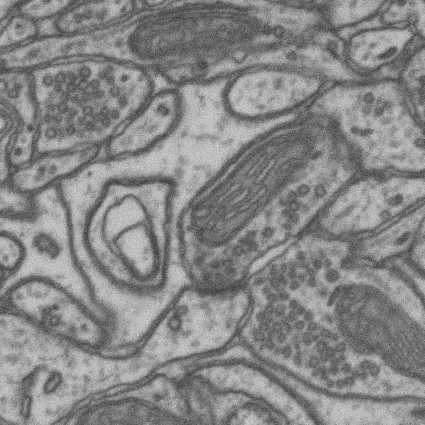
\includegraphics[width=0.9\textwidth]{original_slice.png}
            \caption{Original XY test slice}
        \end{figure}
    \end{minipage}
    \begin{minipage}{0.49\textwidth}
        \centering
        \begin{figure}
            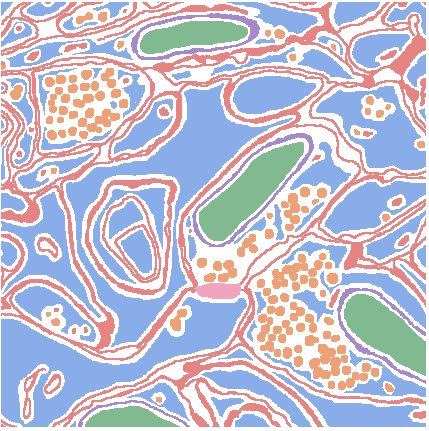
\includegraphics[width=0.9\textwidth]{labeled_slice.png}
            \caption{Labels for the test XY slice}
        \end{figure}
    \end{minipage}
\end{frame}

\begin{frame}
    \frametitle{Distributions of intensities}
    \begin{alertblock}{Are data normally distributed?}
        Statistical test of normality fails, so there is no evidence that data are normally distributed
    \end{alertblock}
    \begin{minipage}{0.49\textwidth}
        \centering
        \begin{figure}
            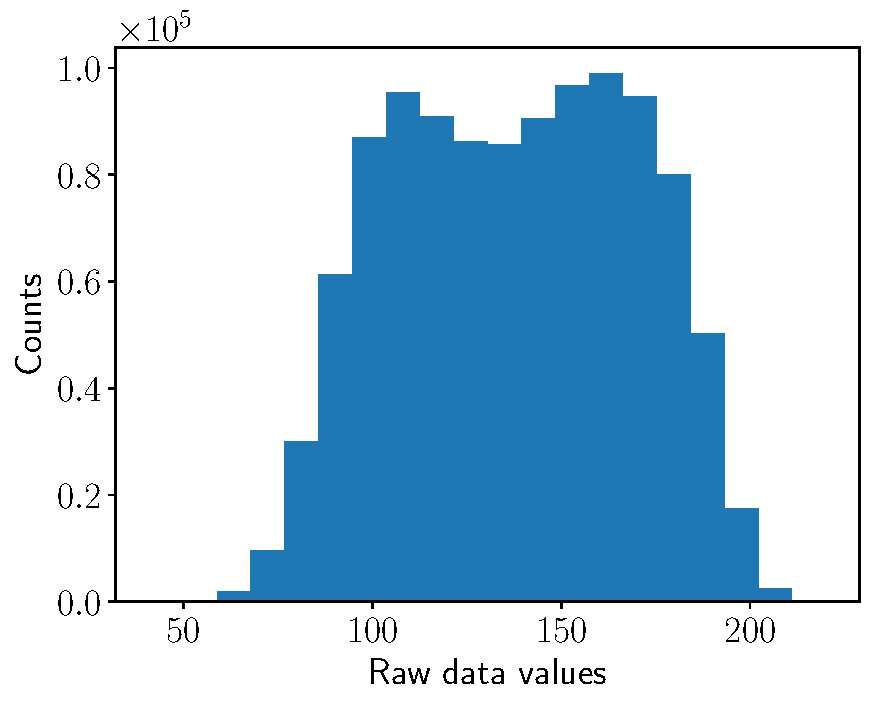
\includegraphics[width=0.9\textwidth]{raw_data_dist.pdf}
            \caption{Connectomics volume image with provided labels}
        \end{figure}
    \end{minipage}
    \begin{minipage}{0.49\textwidth}
        \centering
        \begin{figure}
            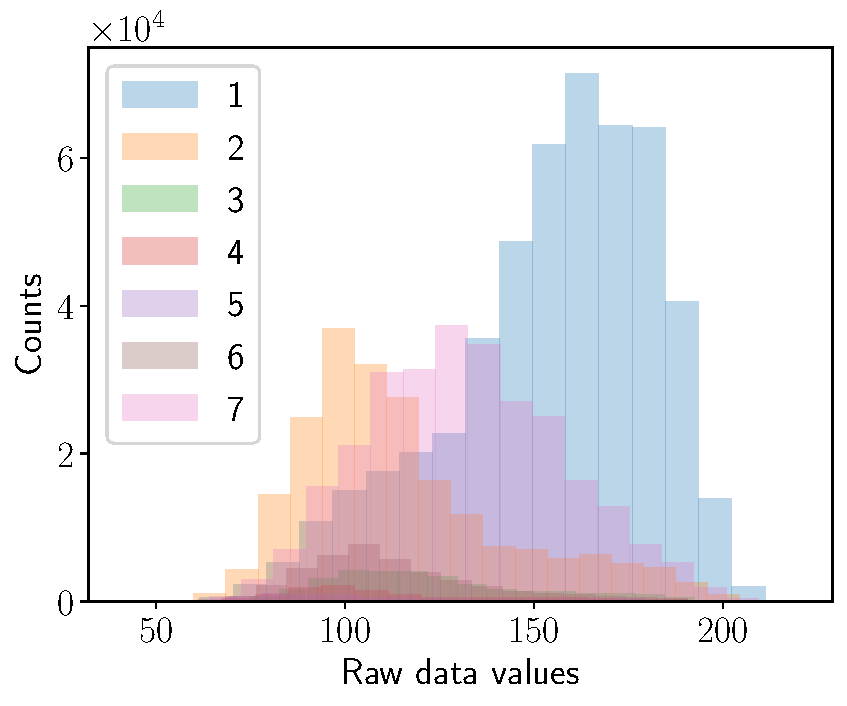
\includegraphics[width=0.9\textwidth]{raw_data_dist_per_label.pdf}
            \caption{Connectomics volume image with provided labels}
        \end{figure}
    \end{minipage}
\end{frame}

\begin{frame}
    \frametitle{Difference in intensities}
    \begin{block}{Means are different}
        Means of all class except cell membrane and mitochondrion membrane are
        different with high confidence levels.
    \end{block}
    \begin{table}[ht]
        \centering
        \begin{tabular}{|c|c|c|c|c|c|c|c| }
            \hline
            Label      & \textbf{1} & \textbf{2} & \textbf{3} & \textbf{4} & \textbf{5} & \textbf{6} & \textbf{7} \\
            \hline
            \textbf{1} & -          & 0          & 0          & 0          & 0          & 0          & 0          \\
            \hline
            \textbf{2} & 0          & -          & 0          & 0.175      & 0          & 0          & 0          \\
            \hline
            \textbf{3} & 0          & 0          & -          & 0          & 0          & 0          & 0          \\
            \hline
            \textbf{4} & 0          & 0.175      & 0          & -          & 0          & 0          & 0.0003     \\
            \hline
            \textbf{5} & 0          & 0          & 0          & 0          & -          & 0          & 0.0029     \\
            \hline
            \textbf{6} & 0          & 0          & 0          & 0          & 0          & -          & 0          \\
            \hline
            \textbf{7} & 0          & 0          & 0          & 0.0003     & 0.0029     & 0          & -          \\
            \hline
        \end{tabular}
        \caption{P-values of t-test for different labels combination}
        \label{tab:data_ttest}
    \end{table}
\end{frame}

\begin{frame}
    \frametitle{Limitations of the dataset}
    \begin{itemize}
        \item Labeling by non expert \textit{\( \Rightarrow \) there may be some mistakes in labeling}
        \item Limited size \textit{(even for artificial data generation via GANs)}
        \item Most interesting and hardest regions are unlabeled
        \item Labels only for slices \textit{\( \Rightarrow \) can not use SOTA segmentation models}
        \item One label per voxel \textit{\( \Rightarrow \) can not perform multi label classification}
        \item High class imbalance
    \end{itemize}
\end{frame}

\section{Methodology}

\begin{frame}
    \frametitle{Voxelwise classification models}

    First of all we evaluate classical ML models where input subvolumes represent only 1 voxel which model should classify
    \linebreak

    \begin{minipage}[t]{0.49\textwidth}
        We use the following ML models:
        \begin{itemize}
            \item Decision tree
            \item Random forest
            \item Ada boosting on trees
            \item Gradient boosting on trees
        \end{itemize}
    \end{minipage}
    \begin{minipage}[t]{0.49\textwidth}
        In addition to intensities we add features computed by filtering and input slice such as:
        \begin{itemize}
            \item Sobel's \(x \) and \(y\) derivatives
            \item Prewitt's \(x \) and \(y\) derivatives
            \item Laplace
            \item Gradient magnitudes from sobel and prewitt gradients
        \end{itemize}
    \end{minipage}
\end{frame}

\begin{frame}
    \frametitle{Convolutional neural networks}

    \begin{minipage}{0.49\textwidth}
        CNN are SOTA models for task like this because they have 2 important advantages over classical models:
        \begin{enumerate}
            \item Downsampling layers reduce dimensionality of features
            \item They learn features and we don't need to invent them by hand
        \end{enumerate}

        All our 6 types of CNNs architectures differ only in backbones.
    \end{minipage}
    \begin{minipage}{0.49\textwidth}
        \begin{figure}
            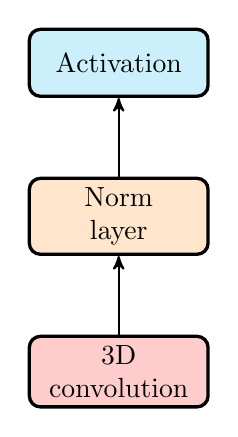
\begin{tikzpicture}[
                    module/.style={draw, very thick, rounded corners, minimum
                            width=15ex},
                    conv/.style={module, minimum height = 0.85cm, fill=red!20},
                    norm/.style={module, minimum height = 0.85cm, fill=orange!20},
                    act/.style={module, minimum height = 0.85cm, fill=cyan!20},
                    arrow/.style={-stealth', thick, rounded corners},
                ]

                \node[conv, align=center] (conv_layer) {3D \\ convolution};
                \node[above=of conv_layer, norm, align=center] (norm_layer) {Norm\\layer};
                \node[above=of norm_layer, act, align=center] (activation) {Activation};

                \draw[arrow] (conv_layer) -- (norm_layer);
                \draw[arrow] (norm_layer) -- (activation);
            \end{tikzpicture}
            \caption{Convolutional block}
            \label{fig:conv_block}
        \end{figure}
    \end{minipage}
\end{frame}

\begin{frame}
    \frametitle{Handcrafted CNN backbones}
\end{frame}

\begin{frame}
    \frametitle{Handcrafted CNN backbones}
\end{frame}

\begin{frame}
    \frametitle{ConvNext}
    We took a SOTA 2D CNN ConvNext \cite{liu2022convnet} and change 2D convolutions with 3D.
    \begin{figure}
        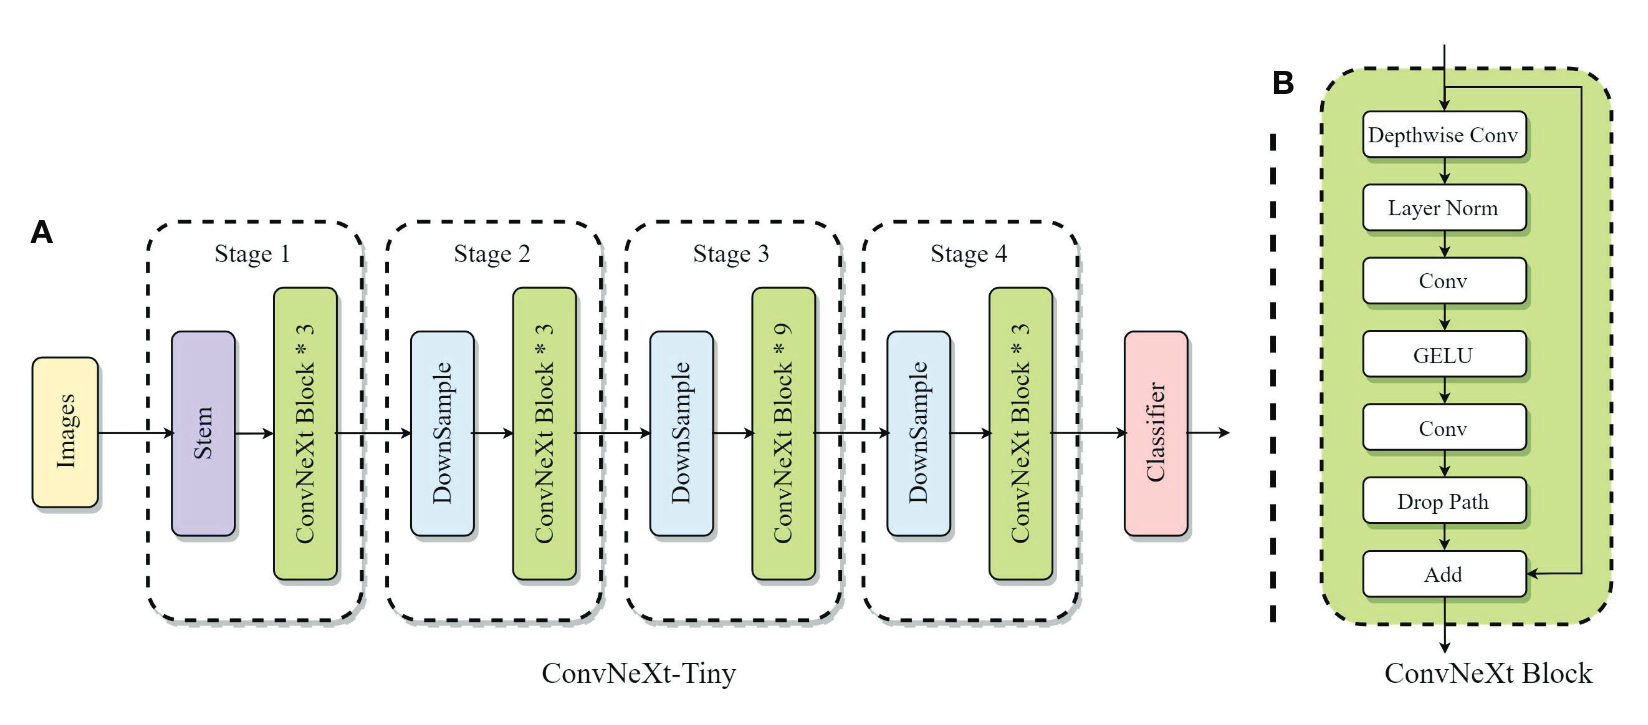
\includegraphics[width=0.8\textwidth]{convnext.png}
        \caption{ConvNext-tiny architecture\footnote{Image source: \url{https://www.researchgate.net/figure/A-ConvNeXt-Tiny-overall-network-structure-B-ConvNeXt-Block-structure_fig2_367224906}}}
    \end{figure}
\end{frame}

\begin{frame}
    \frametitle{Pretraining techniques}



\end{frame}

\begin{frame}
    \frametitle{Tiled predictions}

    \begin{block}{Motivation}
        Predictions for adjacent center voxels share a lot of input data. Can we use
        properties of convolution to reduce number of computation?
    \end{block}

    \begin{minipage}{0.49\textwidth}
        \begin{figure}
            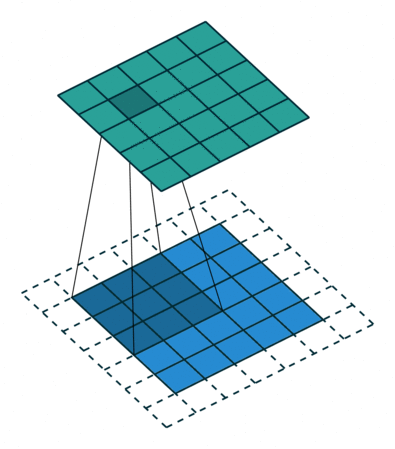
\includegraphics[height=3cm]{conv1.png}
            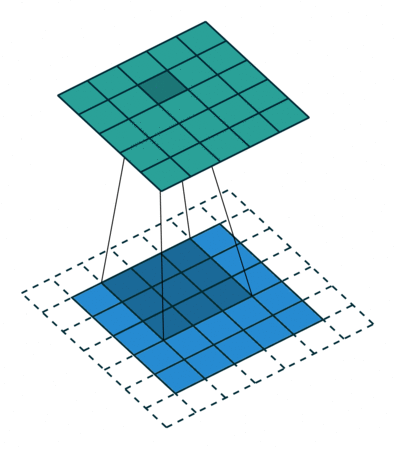
\includegraphics[height=3cm]{conv2.png}
            \caption{Convolution visualization\footnote{Images source: \url{https://towardsdatascience.com/types-of-convolutions-in-deep-learning-717013397f4d}}}
        \end{figure}
    \end{minipage}
    \begin{minipage}{0.49\textwidth}
        Let \( s \) and \( o \) be an standard input and output shape, \( m \) -- additional extent, \( d \) -- downsampling parameter
        \begin{equation*}
            \begin{cases}
                \frac{s + m}{d} = o + m \\
                \frac{s}{d} = o
            \end{cases}
            \implies d = 1
        \end{equation*}

        \begin{alertblock}{No downsampling}
            It is possible iff we don't use any layers with stride \( >1 \)
        \end{alertblock}
    \end{minipage}

\end{frame}

\begin{frame}
    \frametitle{Postprocessing with use of CRF}

    The energy function for CRF is the following:
    \begin{equation*}
        E(\mathbf{x}) =\sum\limits_{i \in V} \theta_i (\mathbf{x_i}) +
        \sum\limits_{ij \in E} \theta_{ij} (\mathbf{x_i}, \mathbf{x_j})
    \end{equation*}
    where \( G = (V, E) \) -- \textbf{complete} graph where every voxel \( v \in V \) is a node,
    \(\mathbf{x}_i\) -- one hot encoding of labeling of the voxel \( i \),
    \( \theta_i = -\ln{p_i} \) -- unary term depended on the predicted probabilities \( p_i \) of labels.

    \begin{equation}  \label{eq:crf_pairwise_term}
        \begin{aligned}
            \theta_{ij} (\mathbf{x_i}, \mathbf{x_j}) = & \mu_1(\mathbf{x_i}, \mathbf{x_j})
            \exp \left( -\frac{\| c_i - c_j \|^2}{2 \theta_{\alpha}^2}
            -\frac{\| I_i - I_j \|^2}{2 \theta_{\beta}^2} \right) +                                                                                            \\
                                                       & \mu_2 (\mathbf{x_i}, \mathbf{x_j}) \exp \left( -\frac{\| c_i - c_j \|^2}{2 \theta_{\gamma}^2} \right)
        \end{aligned}
    \end{equation}
    where \( \mu_k(\mathbf{x_i}, \mathbf{x_j})\)
    -- labels incompatibility term, \( c_i \) -- position of the voxel \( i \),
    \( I_i \in [0, 1] \) -- normalized intensity of voxel \( i \),
    \( \theta_{\alpha}, \theta_{\beta}, \theta_{\gamma}\) -- parameters of the
    importance of corresponding difference in intensity and position.

\end{frame}

\section{Experiments}

\begin{frame}
    \frametitle{Voxelwise models evaluation}
    \begin{table}[ht]
        \centering
        \begin{tabular}{|c|c|c|c|c|c| }
            \hline
            \textbf{Model}                 & \textbf{Features} & \textbf{F1}    & \textbf{AP}    & \( \mathbf{\varkappa} \) \\
            \hline
            \multirow{2}{*}{Decision tree} & 1                 & 0.278          & 0.345          & 0.656                    \\
                                           & 8                 & 0.317          & 0.261          & 0.584                    \\
            \hline
            \multirow{2}{*}{Random forest}
                                           & 1                 & 0.278          & 0.345          & 0.655                    \\
                                           & 8                 & \textbf{0.319} & 0.315          & 0.618                    \\
            \hline
            \multirow{2}{*}{AdaBoost}
                                           & 1                 & 0.277          & 0.219          & 0.654                    \\
                                           & 8                 & 0.281          & 0.212          & \textbf{0.671}           \\
            \hline
            \multirow{2}{*}{GradientBoost}
                                           & 1                 & 0.278          & 0.346          & 0.656                    \\
                                           & 8                 & 0.282          & \textbf{0.355} & 0.676                    \\
            \hline
        \end{tabular}
        \caption{Metrics for voxelwise models}
        \label{tab:voxelwise_metrics}
    \end{table}
\end{frame}

\begin{frame}
    \frametitle{CNN models evaluation}
    \begin{table}[ht]
        \centering
        \begin{tabular}{|p{1.2cm}| >{\centering\arraybackslash}p{1cm}|c|c|c|c|c|}
            \hline
            \textbf{Model} & \textbf{Input shape} & \textbf{Loss}          & \textbf{F1}    & \textbf{AP}    & \( \mathbf{\varkappa} \) \\
            \hline
            4res           & 32                   & CE                     & \textbf{0.913} & \textbf{0.962} & \textbf{0.939}           \\
            \hline
            4conv          & 32                   & CE                     & 0.906          & 0.952          & 0.938                    \\
            \hline
            4res\_ln       & 32                   & CE                     & 0.905          & 0.959          & 0.937                    \\
            \hline
            dil            & 32                   & CE                     & 0.885          & 0.95           & 0.923                    \\
            \hline
            4res           & 16                   & CE                     & 0.883          & 0.933          & 0.926                    \\
            \hline
            4res\_ln       & 16                   & CE                     & 0.851          & 0.925          & 0.918                    \\
            \hline
            dil            & 32                   & Focal (\(\gamma = 2\)) & 0.828          & 0.886          & 0.894                    \\
            \hline
        \end{tabular}
        \caption{Metrics for top 7 CNN models}
        \label{tab:cnn_raw_metrics}
    \end{table}
\end{frame}

\begin{frame}
    \frametitle{Efficiency of pretraining}
    \begin{table}[ht]
        \centering
        \begin{tabular}{|c| >{\centering\arraybackslash}p{1cm}|c|c|c| }
            \hline
            \textbf{Model}            & \textbf{Pretr. type} & \textbf{Input shape} & \textbf{Loss}        & \textbf{F1}    \\
            \hline
            \multirow{3}{*}{ConvNext} & CR1                  & \multirow{3}{*}{32}  & CE                   & \textbf{0.741} \\
                                      & CR0                  &                      & CE                   & 0.682          \\
                                      & -                    &                      & CE                   & 0.701          \\
            \hline
            \multirow{3}{*}{ConvNext} & CR0                  & \multirow{3}{*}{32 } & Focal (\(\gamma=2\)) & \textbf{0.687} \\
                                      & -                    &                      & Focal (\(\gamma=2\)) & 0.531          \\
                                      & -                    &                      & Focal (\(\gamma=4\)) & 0.492          \\
            \hline
            \multirow{2}{*}{ConvNext} & CR1                  & \multirow{2}{*}{16 } & CE                   & 0.603          \\
                                      & -                    &                      & CE                   & \textbf{0.728} \\
            \hline
        \end{tabular}
        \caption{Comparison of ConvNext models with and without pretraining. CR\(N\) means center voxel regression
            with padding equals to \(N\)}
        \label{tab:pretraining_comparison}
    \end{table}
\end{frame}

\begin{frame}
    \frametitle{Quality of postprocessing: metrics}
    \begin{table}[ht]
        \centering
        \begin{tabular}{|p{1.2cm}| >{\centering\arraybackslash}p{1cm}|c|c|c|c|}
            \hline
            \textbf{Model} & \textbf{Input shape} & \textbf{Loss}          & \textbf{F1}                      & \( \mathbf{\varkappa} \)     \\
            \hline
            4res           & 32                   & CE                     & 0.901 \fall{-0.012}              & \textbf{0.937} \fall{-0.002} \\
            \hline
            4conv          & 32                   & CE                     & \textbf{0.902} \fall{-0.004}     & 0.935 \fall{-0.003}          \\
            \hline
            4res\_ln       & 32                   & CE                     & 0.897  \fall{-0.008}             & 0.930 \fall{-0.007}          \\
            \hline
            dil            & 32                   & CE                     & 0.828  \fall{-0.057}             & 0.868 \fall{-0.064}          \\
            \hline
            4res           & 16                   & CE                     & 0.878  \fall{-0.005}             & 0.922 \fall{-0.004}          \\
            \hline
            4res\_ln       & 16                   & CE                     & 0.846  \fall{-0.005}             & 0.916  \fall{-0.002}         \\
            \hline
            dil            & 32                   & Focal (\(\gamma = 2\)) & 0.828  \quad \textcolor{gray}{0} & 0.893  \fall{-0.001}         \\
            \hline
        \end{tabular}
        \caption{Metrics for postprpocesed outputs of top 7 CNN models. The difference with
            metrics for raw prediction are denoted right of the metric values}
        \label{tab:cnn_crf_metrics}
    \end{table}
\end{frame}

\begin{frame}
    \frametitle{Quality of postprocessing: biological structures}
    \begin{minipage}{0.49\textwidth}
        \begin{figure}
            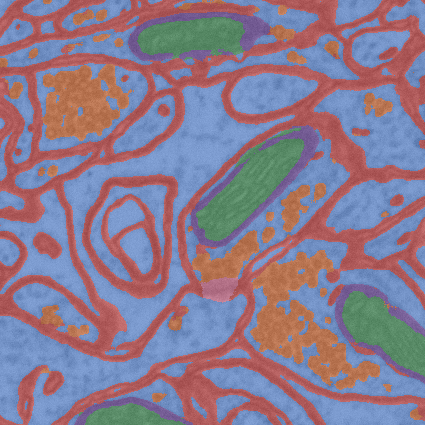
\includegraphics[width=0.9\textwidth]{raw_pred.png}
            \caption{raw predictions}
        \end{figure}
    \end{minipage}
    \begin{minipage}{0.49\textwidth}
        \begin{figure}
            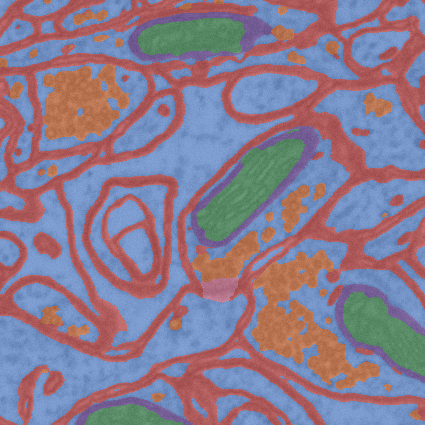
\includegraphics[width=0.9\textwidth]{crf_pred.png}
            \caption{CRF postprpocesed}
        \end{figure}
    \end{minipage}
\end{frame}

\section{Directions of further research}
\begin{frame}
    \frametitle{Context free grammars}
    \begin{minipage}{0.49\textwidth}
        CFGs describe structural properties of the text.

        For example the grammar for balanced parentheses in the Chomsky normal form
        is the following:
        \begin{itemize}
            \item \( S \to SS | LR \)
            \item \( L \to aS | a \)
            \item \( R \to Sb | b \)
            \item \( a \to ( \)
            \item \( b \to \;) \)
        \end{itemize}
    \end{minipage}
    \begin{minipage}{0.49\textwidth}
        \begin{figure}
            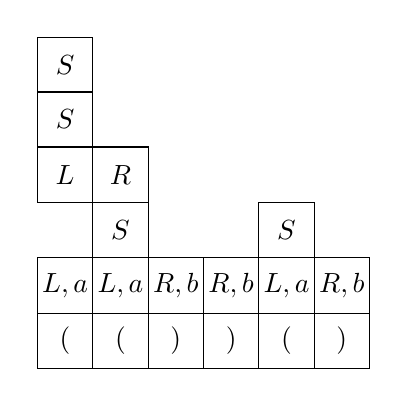
\begin{tikzpicture}
                \matrix[matrix of math nodes, ampersand replacement=\&]
                {
                    S           \&             \&             \&             \&   \&   \\
                    \varnothing \& \varnothing \&             \&             \&   \&   \\
                    S           \& \varnothing \& \varnothing \&             \&   \&   \\
                    L \& R \& \varnothing \& \varnothing \&   \&                       \\
                    \varnothing \& S \& \varnothing \& \varnothing \& S \&             \\
                    L,a \& L,a           \& R,b \& R, b \& L, a \& R,b                 \\
                    (           \& (           \& )           \& )           \& ( \& ) \\
                };
            \end{tikzpicture}
            \caption{Example of the CYK algorithm for CFG for balanced parentheses}
        \end{figure}
    \end{minipage}
\end{frame}

\begin{frame}
    \frametitle{N-dimensional CFGs}
    \cite{schlesinger2013ten} proposed an extension of CFGs and CYK for N dimensional case. We can try to use it
    for connectomics:
    \begin{itemize}
        \item To check the structural validity of the predictions
        \item For refining / training: let's make a stochastic grammar and in a case of fail backtrace to
              voxels that broke the structure and correct them
    \end{itemize}
    \begin{alertblock}{Problem of intractablility}
        The main problem in this regard is to come up with grammar for connectomics, because the
        number of rules grows very fast with increasing an input size
    \end{alertblock}
\end{frame}

\section*{Conclusion}

\begin{frame}
    \frametitle{Conclusions}

    \begin{itemize}
        \item[$\blacksquare$] Using of CNNs is reasonable
        \item[$\blacksquare$] Relatively small residual networks works better than bigger models
        \item[$\blacksquare$] The optimal input shape for used models is \( 32 \times 32 \times 32 \)
        \item[$\blacksquare$] Postprocessing with CRF improves the structural property of predictions
        \item[$\blacksquare$] The computed metrics can not represent real quality of models because of
              unlabeled regions in the dataset
        \item[$\blacksquare$] Segmentation can benefit from involving structural properties of connectomics
              into labeling pipeline
    \end{itemize}

\end{frame}

\section*{References}

\begin{frame}[allowframebreaks]
    \frametitle{References}

    \bibliographystyle{apalike}
    \bibliography{../references.bib}
\end{frame}


\end{document}